\documentclass{beamer}
\usepackage[utf8]{inputenc}
\usepackage[T1]{fontenc}
\usepackage{lmodern}
\usepackage{tikz}
\usetikzlibrary{math}
\usetikzlibrary{snakes}
\usetikzlibrary{decorations.pathreplacing}
\usepackage[absolute,overlay]{textpos}
\usepackage{booktabs}
\usepackage{ulem}
\usepackage{array}

\title{Meilenstein 3}
\author{Projektgruppe FastSense}
\date{25. Januar 2021}

\usecolortheme{seahorse}
\definecolor{dark}{rgb}{0, 0.1, 0.3}
\definecolor{light}{rgb}{0.9, 0.933, 1}
\definecolor{hw}{rgb}{0.8, 1, 0.9}
\definecolor{red}{rgb}{1, 0, 0}
\definecolor{yellow}{rgb}{1, 1, 0}
\definecolor{green}{rgb}{0, 1, 0}
\definecolor{cyan}{rgb}{0, 1, 1}
\definecolor{blue}{rgb}{0, 0, 1}
\definecolor{magenta}{rgb}{1, 0, 1}
\definecolor{grey}{rgb}{0.8, 0.8, 0.8}
\setbeamercolor{normal text}{fg=black}
\setbeamercolor{structure}{fg=dark}
\setbeamercolor{footline}{fg=black}
\setbeamercolor{frametitle}{fg=light,bg=dark}
\setbeamertemplate{itemize items}[circle]
\beamertemplatenavigationsymbolsempty
\addtobeamertemplate{navigation symbols}{}{
    \usebeamerfont{footline}
    \usebeamercolor[fg]{footline}
    {\footnotesize \insertframenumber\\\vspace{0.15cm}}
}
\setbeamertemplate{title page}{
\insertauthor\\\vspace{0.5cm}
\begin{LARGE}\textbf{\inserttitle}\end{LARGE}\\\vspace{0.5cm}
TODO: Bild\\\vspace{0.5cm}
\insertdate
}

\begin{document}

{\setbeamertemplate{navigation symbols}{}
\begin{frame}
\titlepage
\end{frame}}

\begin{frame}{Inhalt}
\tableofcontents
\begin{textblock*}{1cm}(0cm,3.2cm)
\begin{tikzpicture}
\draw [white] (0, 2.35) rectangle +(1, 1); % Hier den y-Wert anpassen, falls sich das Inhaltsverzeichnis noch ändert
\draw [light, ultra thick] (1, 0) -- (7, 0);
\node [right, dark] at (7, 0) {Demonstration};
\end{tikzpicture}
\end{textblock*}
\end{frame}

\section{Recap MS\,2}
\begin{frame}{\secname}
\begin{center}
\begin{tabular}{cc}
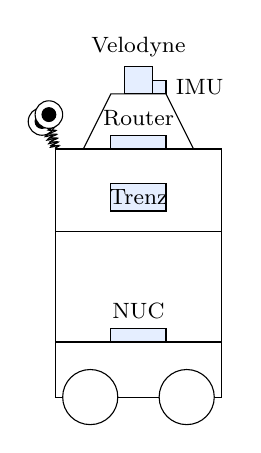
\begin{tikzpicture}[scale=0.35]
\draw (0, 0) rectangle (6, 3);
\draw (1, 3) -- (2, 5) -- (4, 5) -- (5, 3);
\draw [fill=light] (2, 0.75) rectangle +(2, 1);
\node at (3, 1.25) {\footnotesize Trenz};
\draw [fill=light] (2, 3) rectangle +(2, 0.5);
\node [above] at (3, 3.5) {\footnotesize Router};
\draw [fill=light] (2.5, 5) rectangle +(1, 1);
\node [above] at (3, 6) {\footnotesize Velodyne};
\draw (0, 0) -- (0, -6) -- (6, -6) -- (6, 0);
\draw [fill=light] (3.5, 5) rectangle +(0.5, 0.5);
\node [right] at (4, 5.25) {\footnotesize IMU};
\draw (0, -4) -- (6, -4);
\draw [fill=light] (2, -4) rectangle +(2, 0.5);
\node [above] at (3, -3.5) {\footnotesize NUC};
%\draw [fill=light] (2.5, -6) rectangle +(1, 0.5);
%\node [above] at (3, -5.5) {\footnotesize IMU};
\draw [fill=white] (1.25, -6) circle (1);
\draw [fill=white] (4.75, -6) circle (1);
\draw [decorate, decoration={snake, segment length=0.5mm, amplitude=0.5mm}] (-0.5, 4) -- (0, 3);
\draw [fill=white] (-0.5, 4) circle (0.5);
\draw [fill=black] (-0.5, 4) circle (0.25);
\draw [decorate, decoration={snake, segment length=0.5mm, amplitude=0.5mm}] (-0.25, 4.25) -- (0, 3);
\draw [fill=white] (-0.25, 4.25) circle (0.5);
\draw [fill=black] (-0.25, 4.25) circle (0.25);
\end{tikzpicture} &
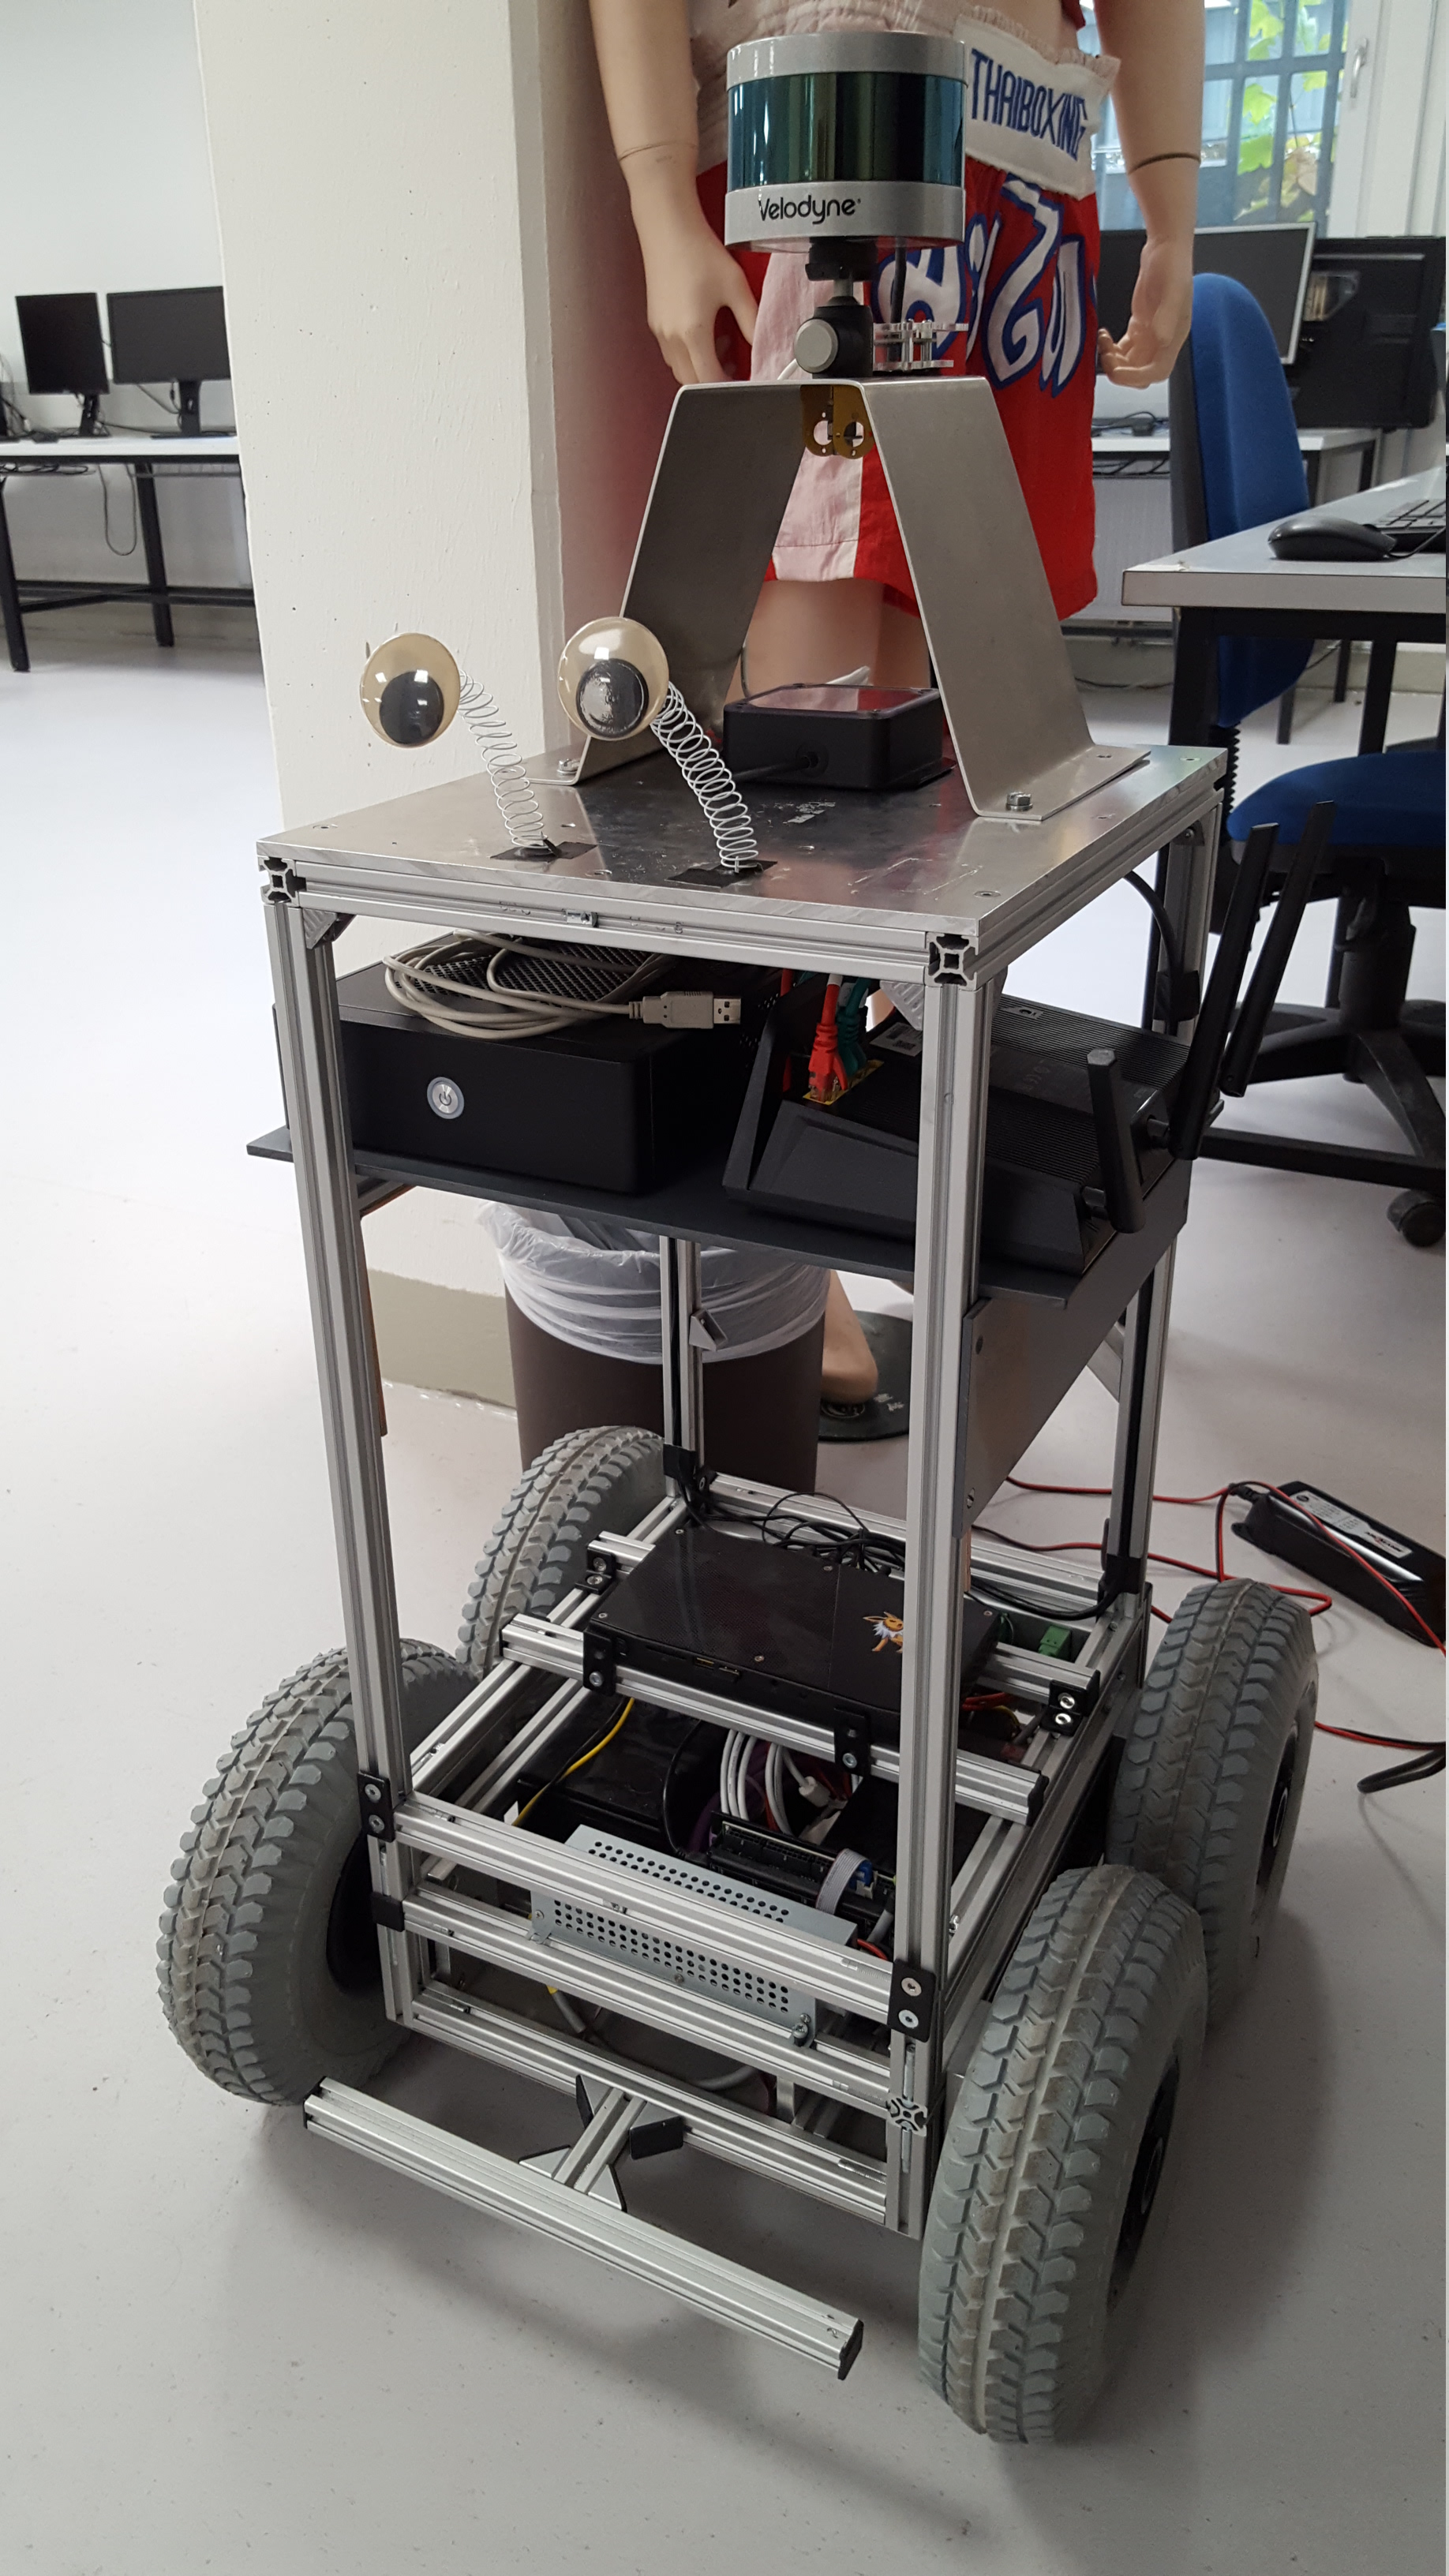
\includegraphics[height=5cm]{images/robot.jpg}
\end{tabular}
\end{center}

\begin{itemize}
\item{Grundlegender Hardware Accelerated TSDF SLAM Algorithmus fertig}
\item{Zeit: 0,87\,fps} % = 1 / (35ms + 676ms + 105ms + 337ms)
\item{Power Consumption: 10,32\,W}
\item{Verbesserungspotenzial vorhanden}
\end{itemize}
\end{frame}

\section{Ziele für MS\,3}
\begin{frame}{\secname}
\begin{textblock*}{12cm}(1cm,2cm)
\begin{itemize}
\item{Aufbau einer SLAM-Box}
\begin{itemize}
\item{Nutzung als Sensor}
\item{Einfache Portierung zwischen Drohne, Roboter, Rucksack etc.}
\item{Festes Interface, einfache Bedienung, Kapselung}
\end{itemize}
\end{itemize}
\end{textblock*}
\begin{textblock*}{12cm}(1cm,3.9cm)
\begin{itemize}
\item{Verbesserung und Optimierung des Algorithmus \\
\vspace{0.2cm}
\begin{tabular}{ll}
\toprule
Variable & Ziel \\
\midrule
Genauigkeit & Wiederfinden erneuter Pose \\
Energie & 0,5\,J/frame \\
Frequenz & \textbf{\color{dark}20\,fps} (echtzeitfähig) \\
Geschwindigkeit & 10\,km/h \\
\bottomrule
\end{tabular}}
\end{itemize}
\end{textblock*}
\begin{textblock*}{12cm}(1cm,7.7cm)
\begin{itemize}
\item{Mesh-Generierung auf Basis der TSDF Werte}
\end{itemize}
\end{textblock*}
\end{frame}

\section{Ergebnisse MS\,3}
\begin{frame}{\secname}
\begin{textblock*}{12cm}(1cm,2cm)
\begin{itemize}
\item{Aufbau einer SLAM-Box {\small\color{dark}$\rightarrow$ \textbf{Aufbau}}}
\begin{itemize}
\item{Nutzung als Sensor}
\item{\sout{Einfache Portierung zwischen Drohne, Roboter, Rucksack etc.}}
\item{Festes Interface, einfache Bedienung, Kapselung}
\end{itemize}
\end{itemize}
\end{textblock*}
\begin{textblock*}{12cm}(1cm,3.9cm)
\begin{itemize}
\item{Verbesserung und Optimierung des Algorithmus}
\begin{itemize}
\item[$\rightarrow$]{\color{dark} \textbf{Base Design}}
\item[$\rightarrow$]{\color{dark} \textbf{Kommunikation}}
\item[$\rightarrow$]{\color{dark} \textbf{Preprocessing}}
\item[$\rightarrow$]{\color{dark} \textbf{Registrierung vollständig auf Hardware}}
\item[$\rightarrow$]{\color{dark} \textbf{Asynchrones TSDF Update}}
\end{itemize}
\end{itemize}
\end{textblock*}
\begin{textblock*}{12cm}(1cm,7.7cm)
\begin{itemize}
\item{Mesh-Generierung auf Basis der TSDF Werte}
\begin{itemize}
\item[$\rightarrow$]{\color{dark} \textbf{Mesh Rekonstruktion}}
\end{itemize}
\end{itemize}
\end{textblock*}
\end{frame}

\subsection{Drohne, Laserscanner}
\begin{frame}{\subsecname}
\begin{itemize}
\item{Drohne erfordert neuen Laserscanner}
\begin{itemize}
\item{Velodyne nicht geeignet}
\end{itemize}
\item{Kontakt mit Firmen:}
\begin{itemize}
\item{Ouster}
\item{Blickfeld}
\end{itemize}
\item[$\rightarrow$]{Future Work}
\end{itemize}
\begin{textblock*}{4cm}(8cm,2cm)
\centering
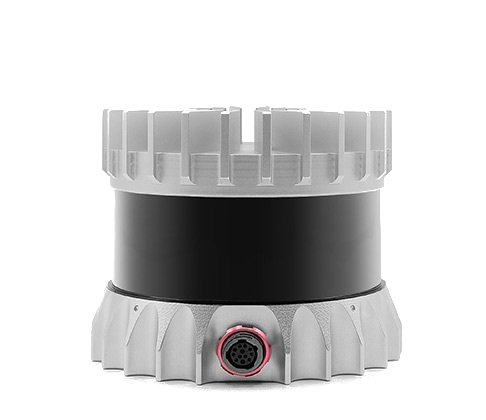
\includegraphics[width=4cm]{images/ouster.png}
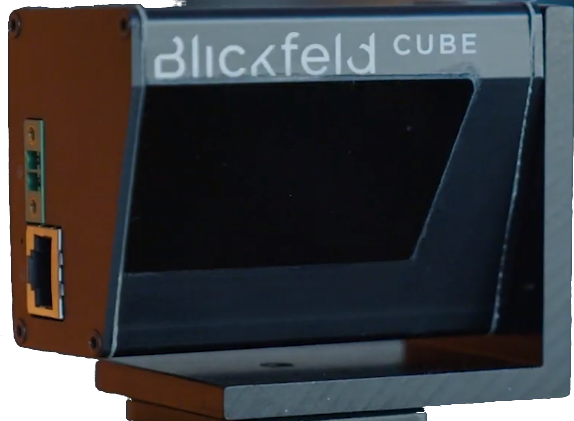
\includegraphics[width=3cm]{images/blickfeld.png}
\end{textblock*}
\end{frame}

\subsection{Aufbau}
\begin{frame}{\subsecname}
\centering
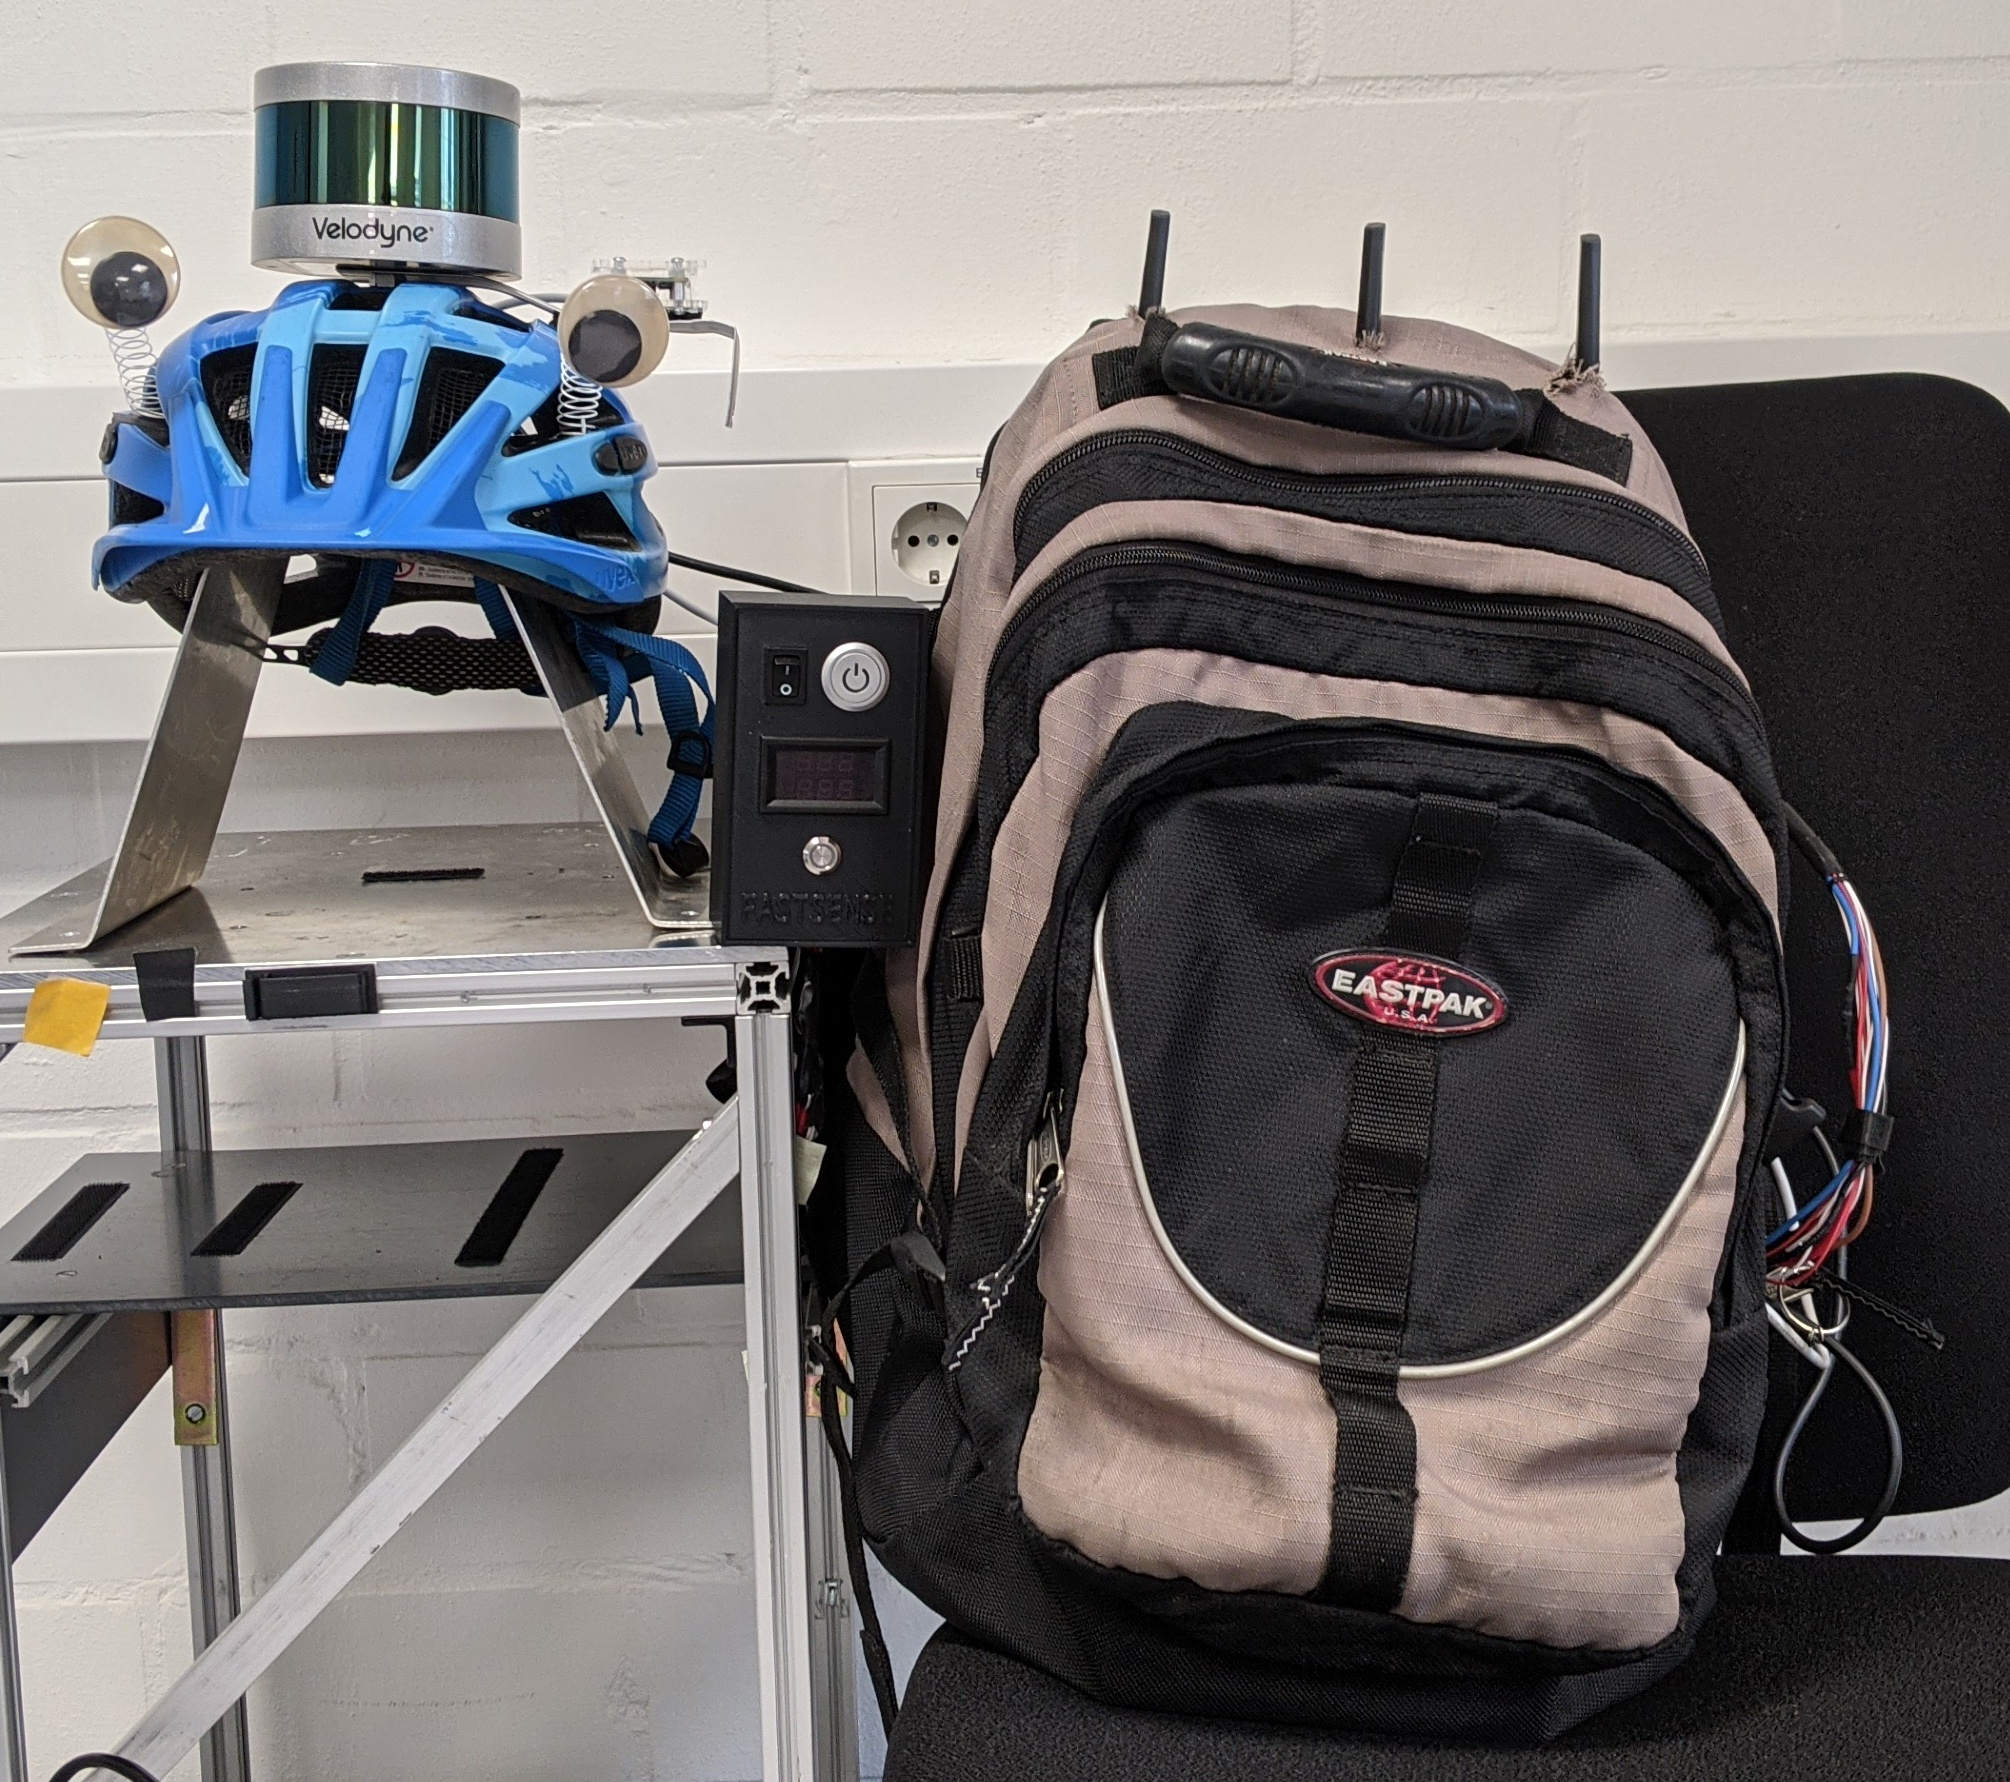
\includegraphics[width=5cm]{images/Rucksack01.jpg}
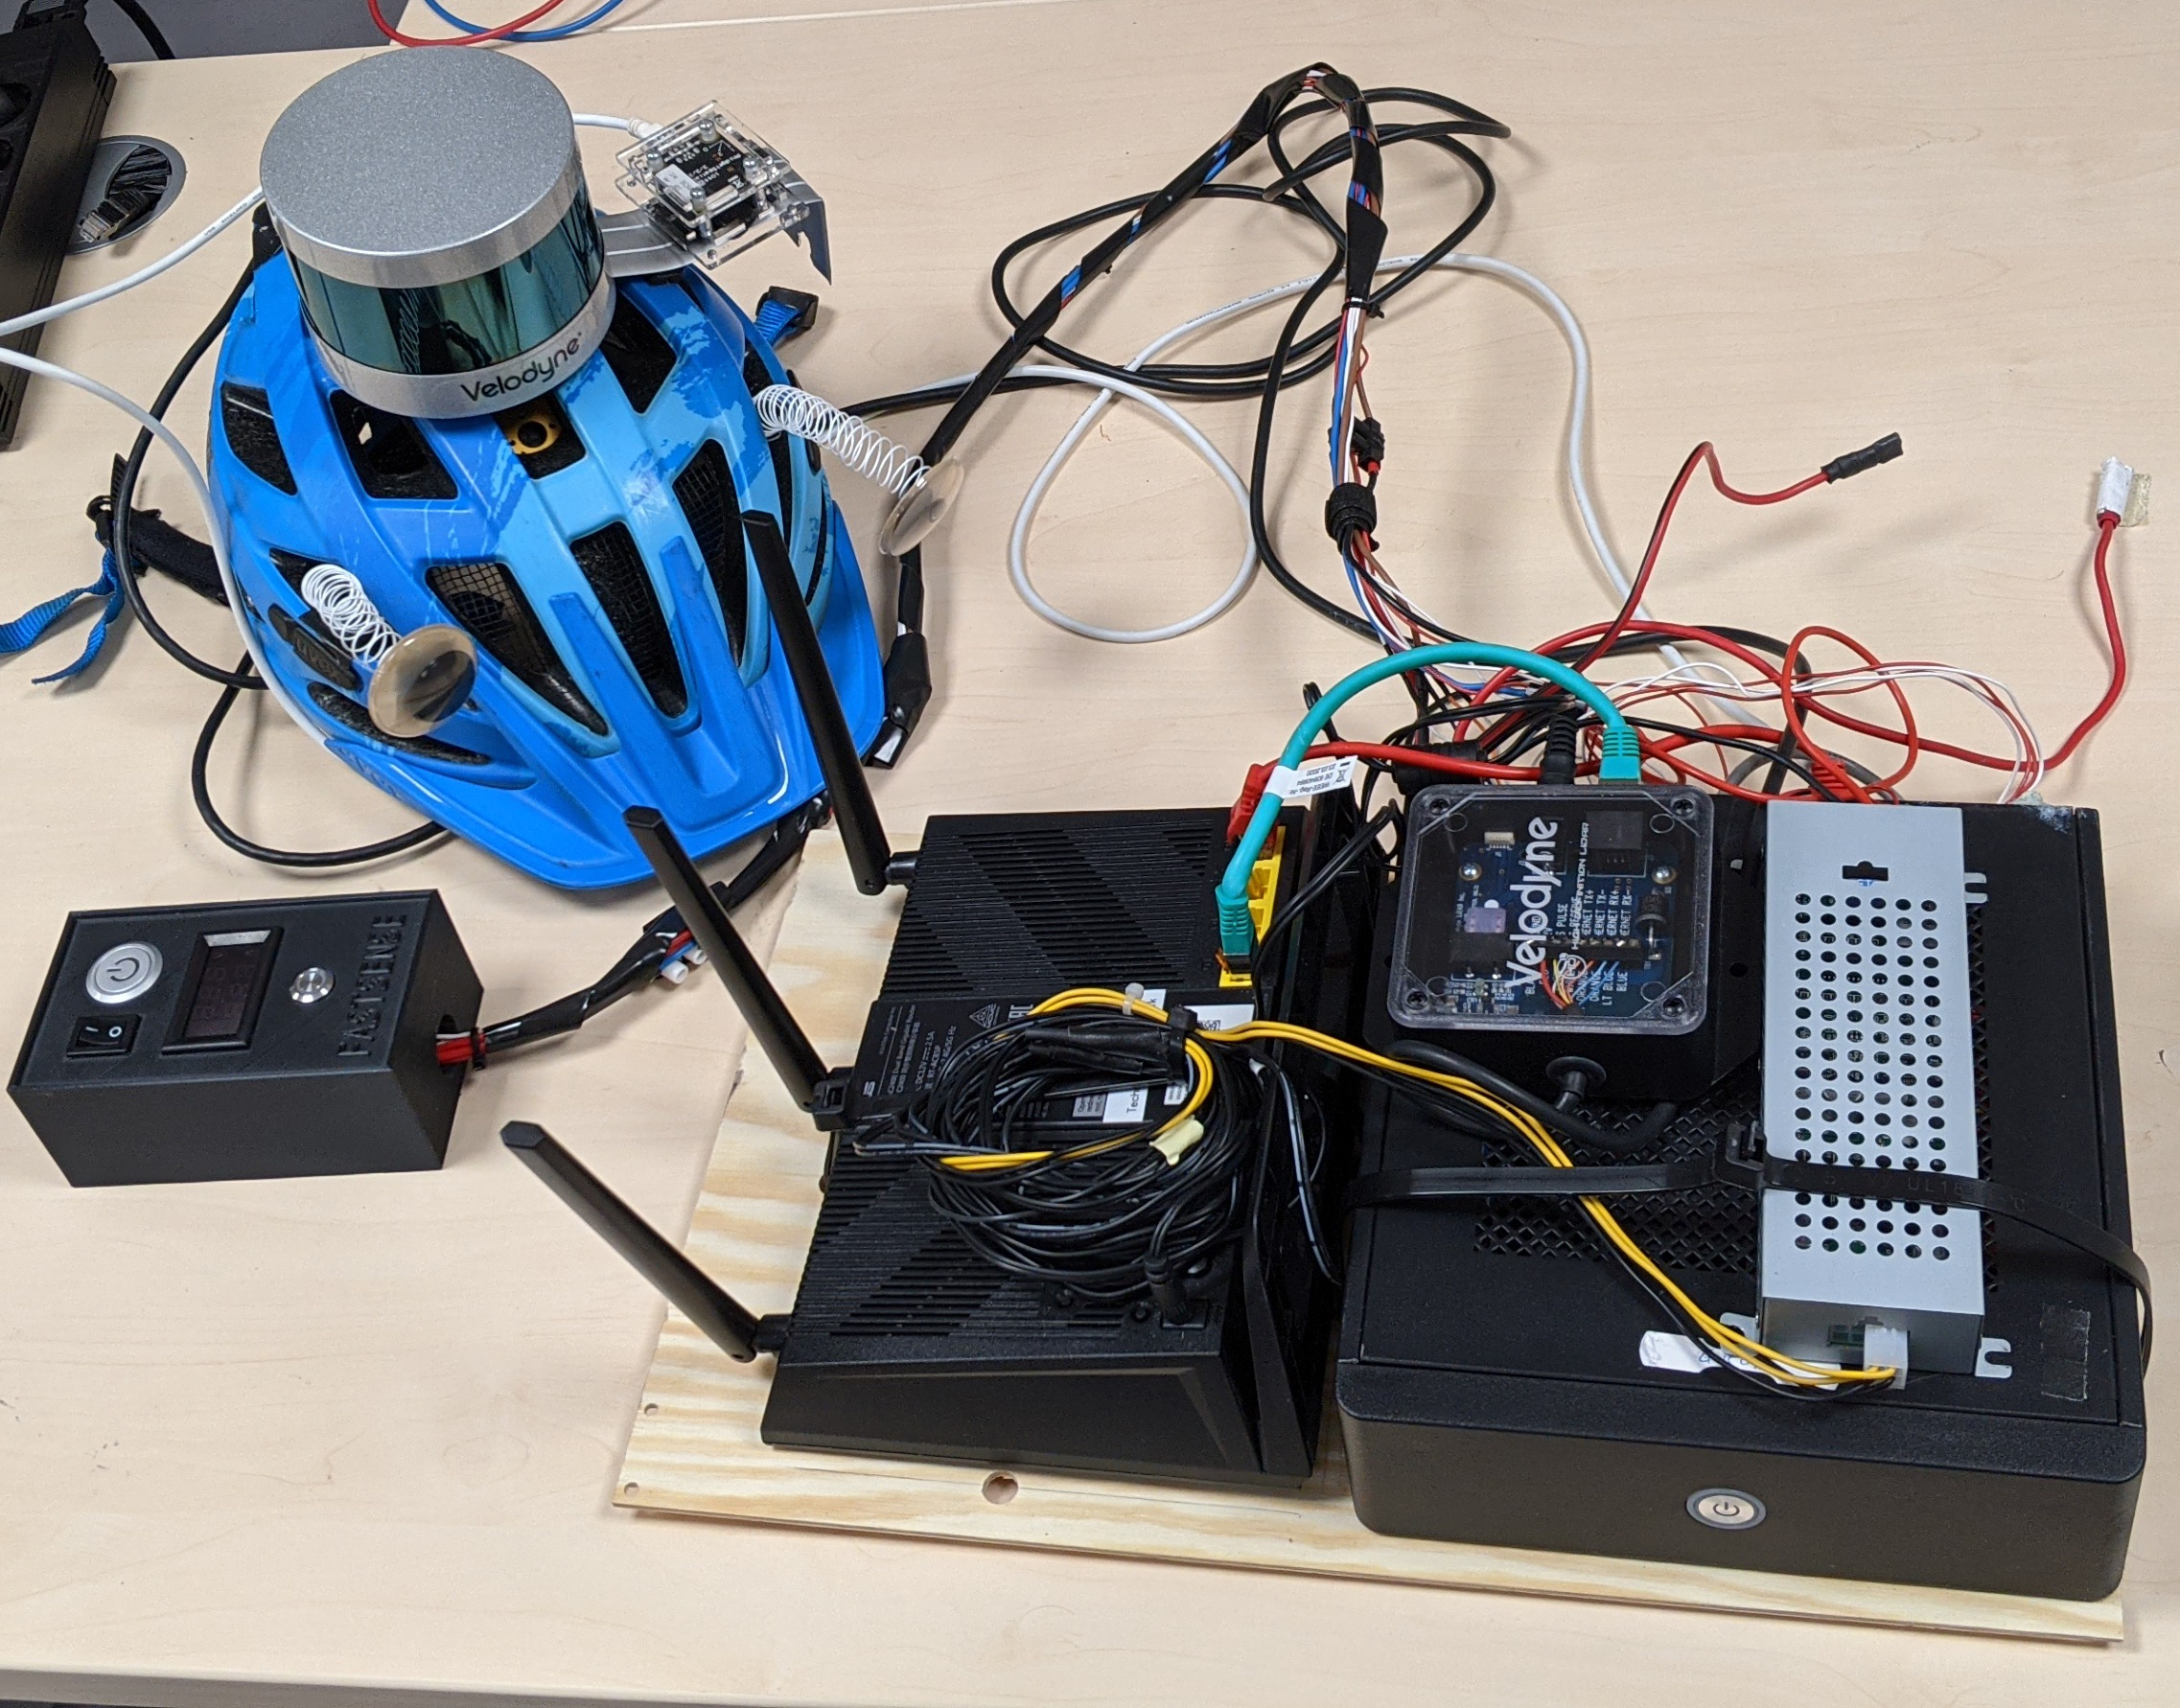
\includegraphics[width=5cm]{images/Rucksack02.jpg}
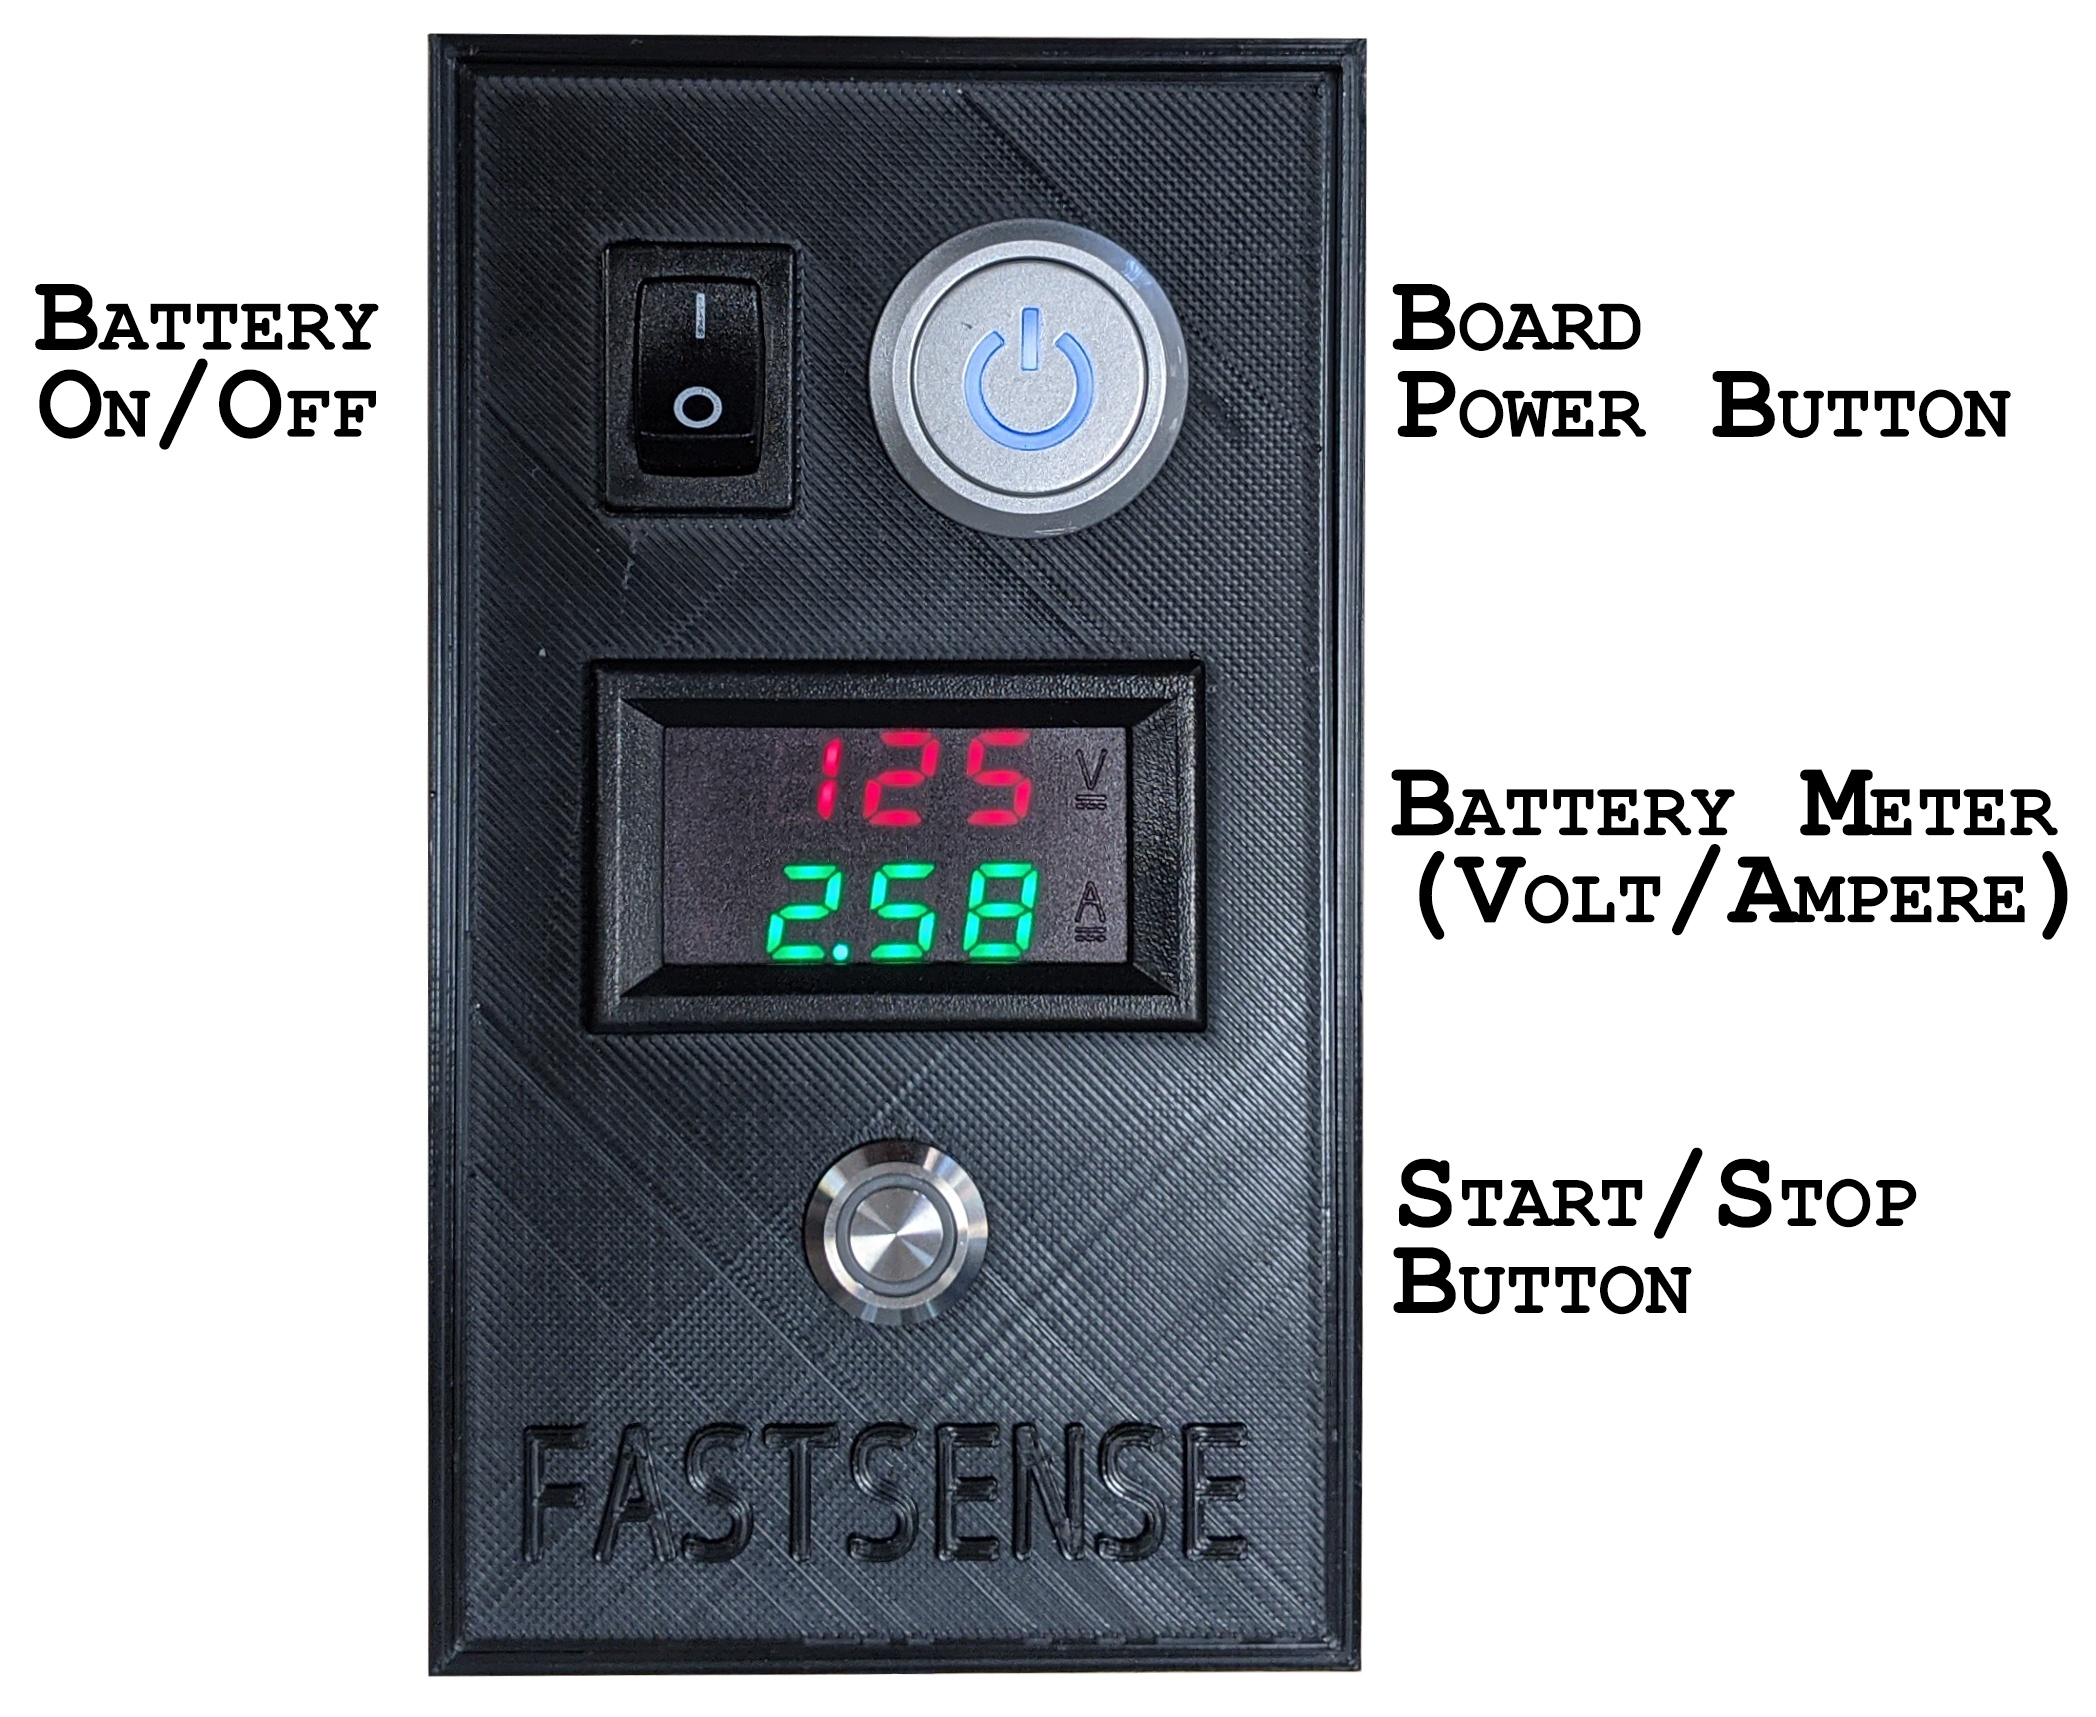
\includegraphics[width=4cm]{images/Box.jpg}
\end{frame}

\subsection{Base Design}
\begin{frame}{\subsecname}
\begin{center}
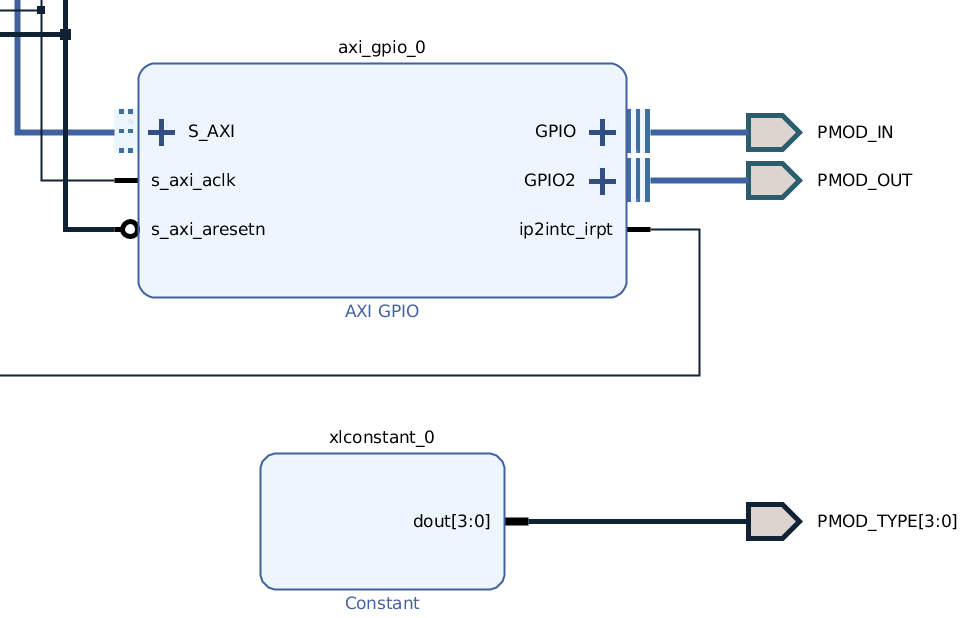
\includegraphics[width=8cm]{images/base_design.png}
\end{center}
\begin{itemize}
\item{GPIO}
\item{Autostart}
\item{Beliebige Taktrate für die Kernel}
\end{itemize}
\end{frame}

\subsection{Kommunikation}
\begin{frame}{\subsecname}
\begin{itemize}
\item{Kommunikation funktioniert in beide Richtungen}
\begin{itemize}
\item[]{\color{dark} Trenz $\rightarrow$ Host (MS02)}
\item[]{\color{dark} Host  \hphantom{} $\rightarrow$ Trenz}
\item[$\rightarrow$]{\color{dark} \textbf{Grundlage für Evaluierung und Reproduzierbarkeit}}
\end{itemize}
\item{Speichern des Poseverlaufs}
\begin{itemize}
\item[$\rightarrow$]{\color{dark} \textbf{Visualisierung der Abweichungen und Pfades in RViz}}
\end{itemize}
\item{Nicht-Blockend}
\begin{itemize}
\item[$\rightarrow$]{\color{dark} \textbf{Sauberes Abspeichern der Global Map}}
\end{itemize}
\end{itemize}
\end{frame}

\subsection{Algorithmus}

\subsubsection*{Preprocessing Punktwolken}
\begin{frame}{\subsecname: \subsubsecname}
\begin{tabular}{m{4cm}m{6cm}}
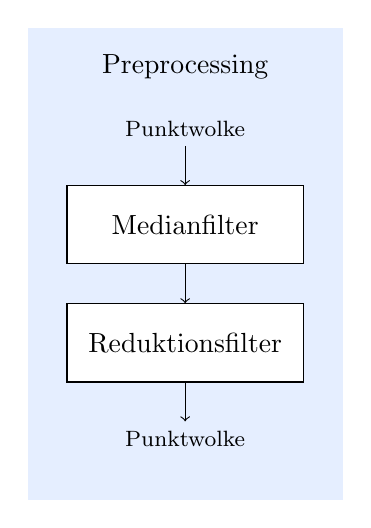
\begin{tikzpicture}
\fill[light] (0, 0) rectangle (4, 6);
\node at (2, 5.5) {Preprocessing};
\draw[->] (2, 4.5) node[above] {\footnotesize Punktwolke} -- (2, 4);
\draw[fill=white] (0.5, 3) rectangle +(3, 1) node[pos=0.5] {Medianfilter};
\draw[->] (2, 3) -- (2, 2.5);
\draw[fill=white] (0.5, 1.5) rectangle +(3, 1) node[pos=0.5] {Reduktionsfilter};
\draw[->] (2, 1.5) -- (2, 1) node[below] {\footnotesize Punktwolke};
\end{tikzpicture} &
\begin{itemize}
\item{Parallelisiert}
\item{Verschiedene Varianten für den Reduktionsfilter}
\begin{itemize}
\item{Average}
\item{Voxel Center}
\item{Random Point}
\item{Closest to Center}
\item[$\rightarrow$]{Kaum Unterschiede}
\end{itemize}
\end{itemize}
\end{tabular}
\end{frame}

\subsubsection*{Preprocessing IMU}
\begin{frame}{\subsecname: \subsubsecname}
\begin{itemize}
\item{Vor Iteration des Algorithmus: Konfigurierbarer Rolling Average Filter}
\item{Während des Algorithmus:\\
Akkumulation bis zur nächsten Punktwolke}
\end{itemize}
\begin{center}
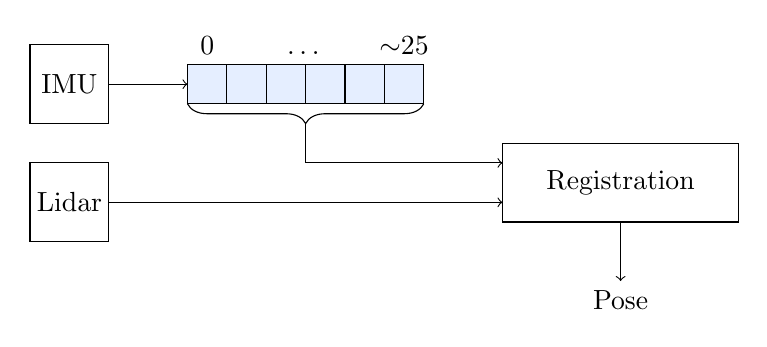
\begin{tikzpicture}
\draw (1, 0) rectangle +(1, 1) node[pos=0.5] {IMU};
\draw[->] (2, 0.5) -- (3, 0.5);
\draw[fill=light] (3, 0.25) rectangle +(3, 0.5);
\node[above] at (3.25, 0.75) {0};
\node[above] at (4.5, 0.75) {\dots};
\node[above] at (5.75, 0.75) {$\sim$25};
\draw (3.5, 0.25) -- (3.5, 0.75);
\draw (4, 0.25) -- (4, 0.75);
\draw (4.5, 0.25) -- (4.5, 0.75);
\draw (5, 0.25) -- (5, 0.75);
\draw (5.5, 0.25) -- (5.5, 0.75);
\draw [decorate, decoration={brace, amplitude=0.25cm, mirror}] (3, 0.25) -- (6, 0.25);
\draw[->] (4.5, 0) -- (4.5, -0.5) -- (7, -0.5);
\draw (7, -1.25) rectangle +(3, 1) node[pos=0.5] {Registration};
\draw (1, -1.5) rectangle +(1, 1) node[pos=0.5] {Lidar};
\draw[->] (2, -1) -- (7, -1);
\draw[->] (8.5, -1.25) -- (8.5, -2) node[below] {Pose};
\end{tikzpicture}
\end{center}
\end{frame}

\subsubsection*{Registrierung}
\begin{frame}{\subsecname: \subsubsecname}
\begin{itemize}
\item[]{\makebox[5cm]{\hfill} 676\,ms}
\item{\makebox[5cm]{Vollständig auf HW\hfill} 74\,ms}
\begin{itemize}
\item{Solver}
\item{Float Matrizen auf HW}
\end{itemize}
\item{Split \& Memports}
\begin{itemize}
\item{\makebox[5cm]{\small Erst 2$\times$\hfill}}\hspace{-\leftmargin} \normalsize 57\,ms
\item{\makebox[5cm]{\small Dann 3$\times$\hfill}}\hspace{-\leftmargin} \normalsize 50\,ms
\end{itemize}
\item{Abbruchkriterium: $\varepsilon$ verändert}
\begin{itemize}
\item{\makebox[5cm]{\small 0,0001 $\rightarrow$ 0,01 \hfill}}\hspace{-\leftmargin} \normalsize 44\,ms
\item{\makebox[5cm]{\small 0,01 $\rightarrow$ 0,04\hfill}}\hspace{-\leftmargin} \normalsize 30\,ms
\end{itemize}
\end{itemize}
\vspace{0.5cm}
\begin{itemize}
\item{Rotation gefixt}
\begin{itemize}
\item{Relativ zum Scanner statt zum Ursprung}
\end{itemize}
\end{itemize}
\end{frame}

\subsubsection*{Asynchronität}
\begin{frame}{\subsecname: \subsubsecname}
\begin{textblock*}{12.8cm}(0cm, 1.5cm)
\centering
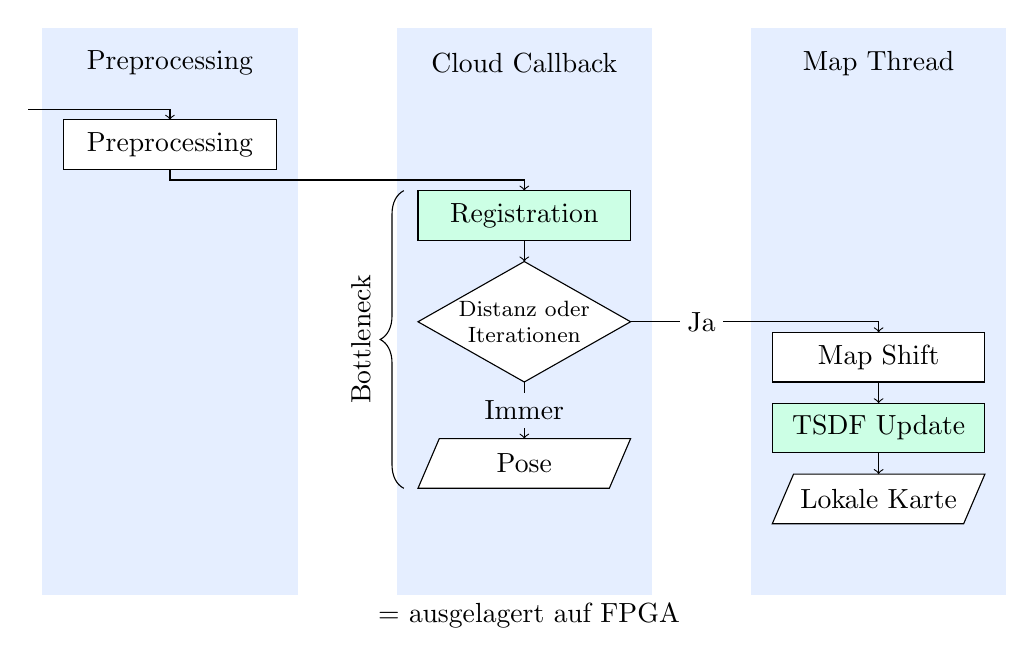
\begin{tikzpicture}[scale=0.9]
\fill[light] (-5.3, 1) rectangle (-1.7, 9);
\fill[light] (-0.3, 1) rectangle (3.3, 9);
\fill[light] (4.7, 1) rectangle (8.3, 9);
\node at (-3.5, 8.5) {Preprocessing};
\node at (1.5, 8.5) {Cloud Callback};
\node at (6.5, 8.5) {Map Thread};
\draw[->] (-5.5, 7.85) -- (-3.5, 7.85) -- (-3.5, 7.7);
\draw[fill=white] (-5, 7) rectangle +(3, 0.7) node[pos=0.5] {Preprocessing};
\draw[->] (1.5, 6) -- (1.5, 5.7);
\draw[fill=hw] (0, 6) rectangle +(3, 0.7) node[pos=0.5] {Registration};
\draw[->] (-3.5, 7) -- (-3.5, 6.85) -- (1.5, 6.85) -- (1.5, 6.7);
\draw[fill=white] (0, 4.85) -- (1.5, 4) -- (3, 4.85) -- (1.5, 5.7) -- cycle;
\node at (1.5, 4.85) {\begin{minipage}{2cm}\centering\footnotesize Distanz oder\\Iterationen\\\end{minipage}};
\draw[->] (1.5, 4) -- (1.5, 3.2) node[midway, fill=light, inner sep=0.1cm] {Immer};
\draw[fill=white] (0, 2.5) -- (2.7, 2.5) -- (3, 3.2) -- (0.3, 3.2) -- cycle;
\node at (1.5, 2.85) {Pose};
\draw[->] (3, 4.85) -- (6.5, 4.85) -- (6.5, 4.7);
\node[fill=white, inner sep=0.1cm] at (4, 4.85) {Ja};
\draw[fill=white] (5, 4) rectangle +(3, 0.7) node[pos=0.5] {Map Shift};
\draw[->] (6.5, 3) -- (6.5, 2.7);
\draw[fill=hw] (5, 3) rectangle +(3, 0.7) node[pos=0.5] {TSDF Update};
\draw[->] (6.5, 4) -- (6.5, 3.7);
\draw[fill=white] (5, 2) -- (7.7, 2) -- (8, 2.7) -- (5.3, 2.7) -- cycle;
\node at (6.5, 2.35) {Lokale Karte};
\draw [decorate, decoration={brace, amplitude=0.3cm, mirror}]
(-0.2, 6.7) -- (-0.2, 2.5) node[midway, xshift=-0.3cm, above, rotate=90] {Bottleneck};
\node at (1.5, 0.7) {{\color{hw}$\blacksquare$} = ausgelagert auf FPGA};
\end{tikzpicture}
\end{textblock*}
\end{frame}

\subsection{Mesh Rekonstruktion}
\begin{frame}{\subsecname}
\begin{itemize}
\item{Global Map offline}
\begin{itemize}
\item{Programm im LVR2 Repository}
\item{Mesh Verbesserungen}
\item{HDF5 $\rightarrow$ PLY}
\end{itemize}
\item{Local Map online}
\begin{itemize}
\item{ROS Node}
\item{Marker Message $\rightarrow$ Mesh Message}
\end{itemize}
\end{itemize}

\begin{center}
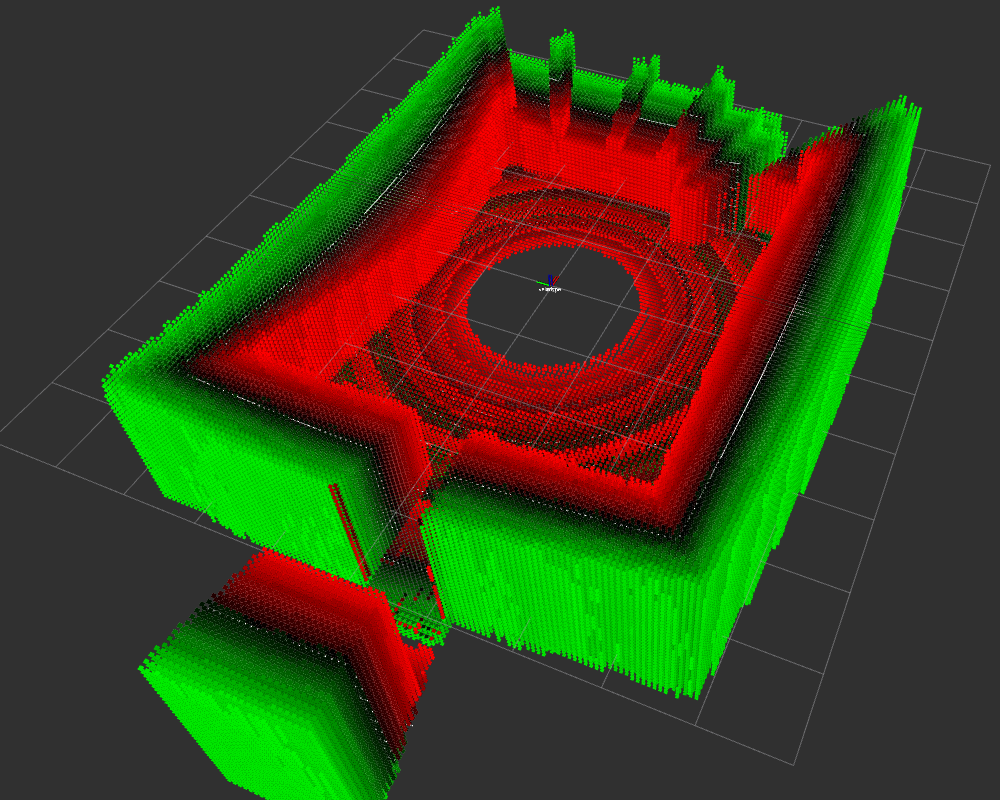
\includegraphics[width=5cm]{images/ReconstructionTSDF.png}
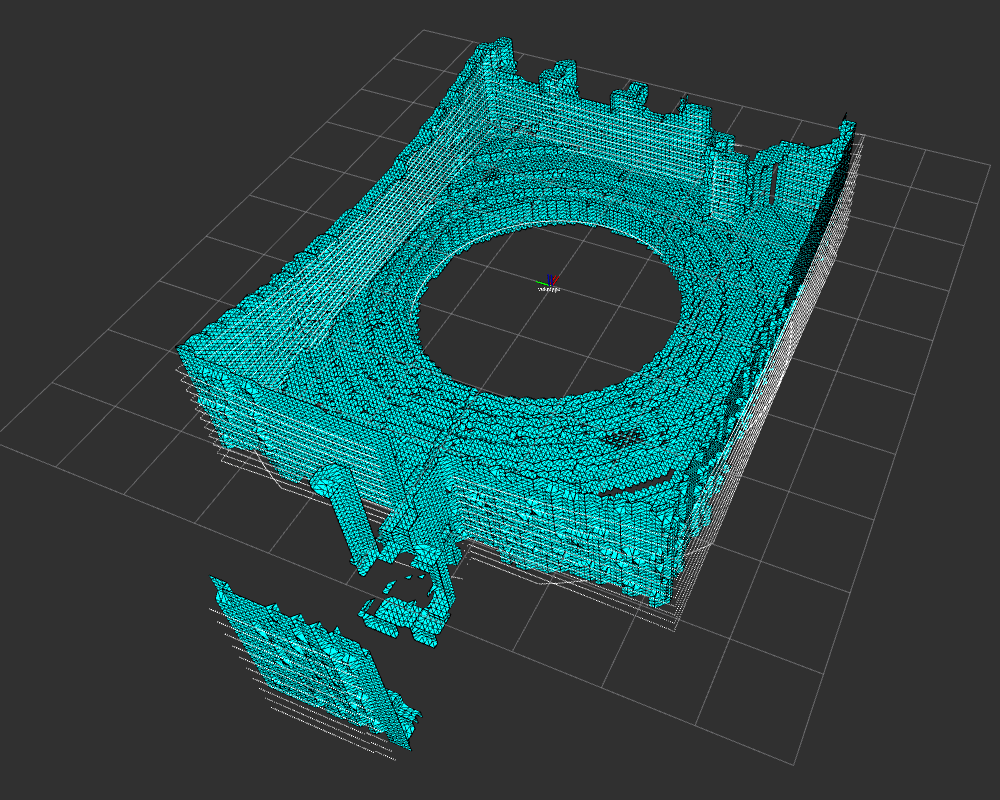
\includegraphics[width=5cm]{images/ReconstructionMesh.png}
\end{center}
\end{frame}

\subsection{Paper}
\begin{frame}{\subsecname}
\centering
\begin{tikzpicture}[scale=0.8]
\draw[thick] (-4, 0) rectangle +(2, 5.4);
\node at (-3, 0.5) {\begin{minipage}{2cm}\centering\footnotesize
External\\
ROS Nodes\\
\end{minipage}};

\draw[fill=light] (-3.8, 3.2) rectangle +(1.6, 2) node[pos=0.5] {\begin{minipage}{1.6cm}\centering
%Sensors\\
%\begin{footnotesize}
%Lidar\\
%IMU\\
%Camera\\
%\dots\\
%\end{footnotesize}
\end{minipage}};

\draw[fill=light] (-3.8, 1) rectangle +(1.6, 2) node[pos=0.5] {\begin{minipage}{1.6cm}\centering
%Control\\
%\begin{footnotesize}
%Motor\\
%Battery\\
%\dots\\
%\end{footnotesize}
\end{minipage}};

\draw (0.2, 1.4) rectangle +(6.4, 3.8);
\node at (3.4, 4.9) {\footnotesize Reconfigurable System on Chip};
\node at (3.56, 0.66) {\includegraphics[height=0.96cm]{images/pynq.png}};
\draw (0.2, 1.4) -- (3.1, 0.7);
\draw (6.6, 1.4) -- (3.7, 0.7);
\draw[dark, ultra thick] (3.4, 0.7) circle (0.3);

\draw[fill=light] (0.4, 1.6) rectangle +(2, 3);
\node at (1.4, 4.1) {\footnotesize Processor};
\draw (0.5, 3.1) rectangle +(1.8, 0.5);% node[pos=0.5] {\footnotesize ROS Master};
\draw (0.5, 2.5) rectangle +(1.8, 0.5);% node[pos=0.5] {\tiny Motor Ctrl Node};
\draw (0.5, 1.9) rectangle +(1.8, 0.5);% node[pos=0.5] {\tiny SLAM Node};
%\node at (1.4, 1.75) {\footnotesize \dots};

\draw[shade, left color=light, right color=hw] (2.6, 1.6) rectangle +(1.6, 3);
\node at (3.4, 4.1) {\begin{minipage}{1.6cm}\centering\footnotesize
Shared\\
Memory\\
\end{minipage}};

\draw[fill=hw] (4.4, 1.6) rectangle +(2, 3);
\node at (5.4, 4.1) {\footnotesize FPGA};

\node at (-1, 3.1) {\begin{minipage}{2cm}\centering\footnotesize
ROS\\
Messages\\
\end{minipage}};
\draw[<->] (-2.2, 3.8) -- (0.4, 3.8);
\draw[<->] (-2.2, 2.4) -- (0.4, 2.4);

\draw[thick] (0, 0) rectangle +(6.8, 5.4);
\node[left] at (6.8, 0.3) {\footnotesize ReconfROS};

% Shared Memory
\draw (2.9, 3.15) rectangle +(1, 0.4);
\draw (2.9, 2.55) rectangle +(1, 0.4);
\draw (2.9, 1.95) rectangle +(1, 0.4);

% FPGA
\draw (4.5, 3.1) rectangle +(1.8, 0.5);% node[pos=0.5] {\tiny Path Detection};
\draw (4.5, 2.5) rectangle +(1.8, 0.5);% node[pos=0.5] {\tiny Registration};
\draw (4.5, 1.9) rectangle +(1.8, 0.5);% node[pos=0.5] {\tiny Outlier Removal};
%\node at (5.4, 1.75) {\footnotesize \dots};

\draw[<->] (2.3, 2.75) -- (2.9, 3.35);
\draw[<->] (2.3, 2.15) -- (2.9, 2.75);
\draw[<->] (2.3, 2.15) -- (2.9, 2.15);
\draw[<->] (3.9, 3.35) -- (4.5, 3.35);
\draw[<->] (3.9, 2.75) -- (4.5, 2.75);
\draw[<->] (3.9, 2.15) -- (4.5, 2.15);
\end{tikzpicture}

\vspace{0.3cm}

\begin{tikzpicture}[scale=0.7]
\setlength{\fboxsep}{0pt}
\node[inner sep=0pt] at (0, 5) {\fbox{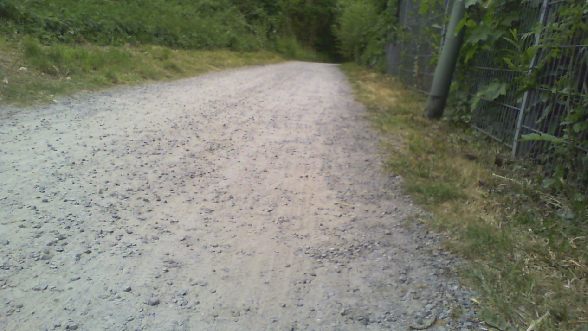
\includegraphics[width=2.1cm]{images/pipeline_pics/cam.png}}};
\node at (0, 3.75) {\footnotesize Camera image};
\node[inner sep=0pt] at (4, 5) {\fbox{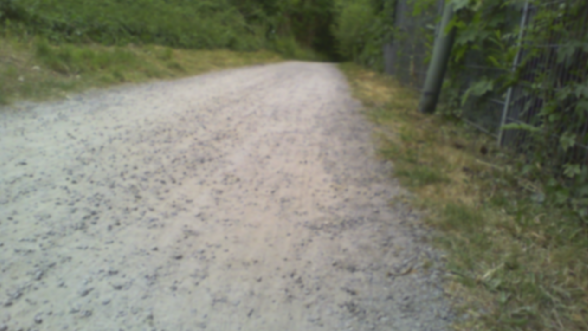
\includegraphics[width=2.1cm]{images/pipeline_pics/gauss.png}}};
\node at (4, 3.75) {\footnotesize Removing noise};
\node[inner sep=0pt] at (8, 5) {\fbox{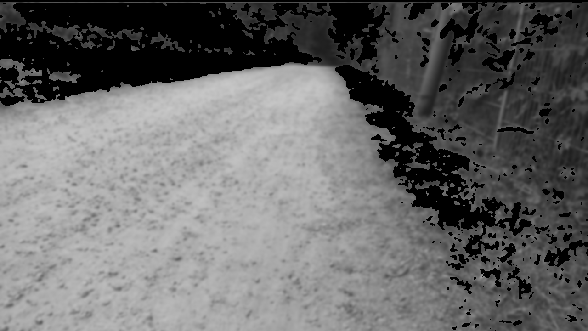
\includegraphics[width=2.1cm]{images/pipeline_pics/green_filter.png}}};
\node at (8, 3.75) {\footnotesize Trail pixel extraction};
\node[inner sep=0pt] at (0, 2) {\fbox{
\includegraphics[width=2.1cm]{images/pipeline_pics/threshold.png}}};
\node at (0, 0.75) {\footnotesize Thresholding};
\node[inner sep=0pt] at (4, 2) {\fbox{
\includegraphics[width=2.1cm]{images/pipeline_pics/morph.png}}};
\node at (4, 0.75) {\footnotesize Remove fragments};
\node[inner sep=0pt] at (8, 2) {\fbox{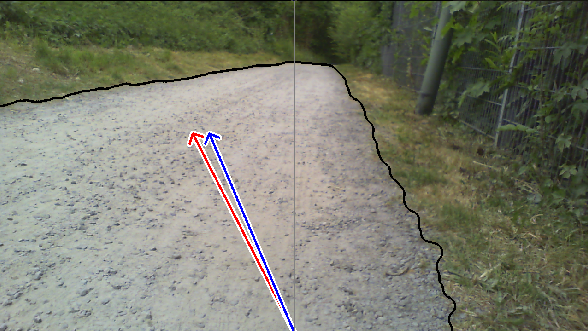
\includegraphics[width=2.1cm]{images/pipeline_pics/direction.png}}};
\node at (8, 0.75) {\footnotesize Trail direction};
\draw[->] (1.5, 5) -- (2.5, 5);
\draw[->] (5.5, 5) -- (6.5, 5);
\draw[->] (9.5, 5) -- (10, 5) -- (10, 3.25) -- (-2, 3.25) -- (-2, 2) -- (-1.5, 2);
\draw[->] (1.5, 2) -- (2.5, 2);
\draw[->] (5.5, 2) -- (6.5, 2);
\end{tikzpicture}
\end{frame}

\section{Evaluation}

\subsection{Zeit}
\begin{frame}{\secname: \subsecname}
\begin{textblock*}{12.8cm}(0cm, 2.5cm)
\centering
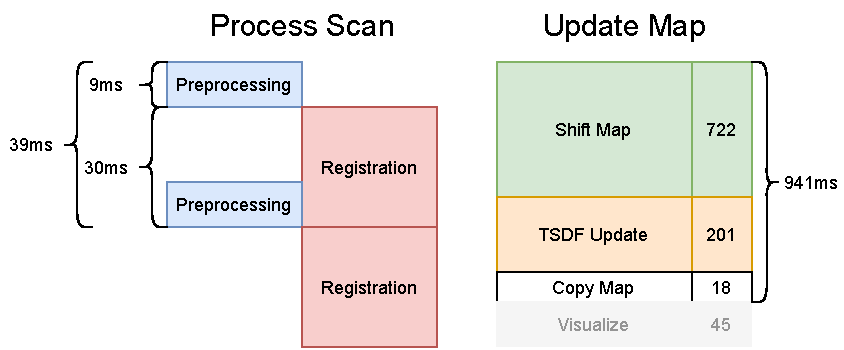
\includegraphics[width=12cm]{images/Zeiten.pdf}
\end{textblock*}
\end{frame}

\begin{frame}{\secname: \subsecname}
\begin{textblock*}{12.8cm}(0cm, 1.1cm)
\centering
\definecolor{bad}{rgb}{1, 0.5, 0.4}
\begin{tikzpicture}[scale=0.85]
\draw[->] (0, 0) -- (10.5, 0) node[right] {Zeit [ms]};
\draw[->] (0, 0) -- (0, 8) node[above] {Anzahl Frames};
\foreach \i\y in {0/3,1/11,2/15,3/10,4/7,5/3,6/2,7/1,8/1,9/1} {
    \pgfmathsetmacro\x{int(\i * 10)}
    \draw (\i, -0.1) node[below]{\x} -- (\i, 0.1);
    \tikzmath {
        if {\i < 5} then {
            let \c = light;
        } else {
            let \c = bad;
        };
        { \draw[fill=\c] (\i, 0) rectangle (\i+1, \y/2); };
    }
}
\draw (9.5, 0.25) -- (9.5, -0.5) node[below] {$>90$};
\node at (9.5, 5) {\begin{minipage}{5.5cm}
\begin{itemize}
\item{Avg: 30ms}
\item[\color{bad}$\bullet$]{11\% aller Scans über 50\,ms}
\item[\color{red}$\bullet$]{2\% gedroppt}
\end{itemize}
\end{minipage}};
\end{tikzpicture}
\end{textblock*}
\end{frame}

\begin{frame}{\secname: \subsecname}
\begin{textblock*}{12.8cm}(0cm, 1.1cm)
\centering
\definecolor{bad}{rgb}{1, 0.5, 0.4}
\begin{tikzpicture}[scale=0.85]
\draw[->] (0, 0) -- (10.5, 0) node[right] {Zeit [ms]};
\draw[->] (0, 0) -- (0, 8) node[above] {Anzahl Frames};
\foreach \i\y in {0/1,1/5,2/7,3/8,4/8,5/14,6/7,7/3,8/1,9/2} {
    \pgfmathsetmacro\x{int(\i * 10)}
    \draw (\i, -0.1) node[below]{\x} -- (\i, 0.1);
    \tikzmath {
        if {\i < 5} then {
            let \c = light;
        } else {
            let \c = bad;
        };
        { \draw[fill=\c] (\i, 0) rectangle (\i+1, \y/2); };
    }
}
\draw (9.5, 0.25) -- (9.5, -0.5) node[below] {$>90$};
\node at (9.5, 5) {\begin{minipage}{5.5cm}
\begin{itemize}
\item{Vergleich: $\varepsilon = 0.01$}
\item{Avg: 47ms}
\item[\color{bad}$\bullet$]{48\% aller Scans über 50\,ms}
\item[\color{red}$\bullet$]{10\% gedroppt $\Rightarrow$ 18 fps}
\end{itemize}
\end{minipage}};
\end{tikzpicture}
\end{textblock*}
\end{frame}

\subsection{Power Consumption}
\begin{frame}{\secname: \subsecname}
TODO: Adrian
\end{frame}

\subsection{Qualität}
\begin{frame}{\secname: \subsecname}
\begin{itemize}
\item{6. Stockwerk (Distanzabweichung in Meter)}
\begin{center}
\begin{tabular}{ |c|c|c| }
    \hline
    epsilon & 0.01 & 0.04 \\ 
    \hline
    & 0.0615 & 0.0505 \\  
    \hline
\end{tabular}
\end{center}
\begin{center}
\begin{tabular}{ |c|c|c| }
    \hline
    Geschw. & langsam & schnell \\ 
    \hline
    & 0.0505 & 0.0437 \\  
    \hline
\end{tabular}
\end{center}
\begin{itemize}
    \item{gesamt (langsam, epsilon = 0.04): 0.075349}
\end{itemize}
\item{8 Meter Labortest (Distanzabweichung in Meter)}
\begin{center}
\begin{tabular}{ |c|c|c|c| }
    \hline
    & hin & zurück & gesamt \\ 
    \hline
    langsam & 0.0548 & 0.0650 & 0.0861 \\  
    schnell & 0.1676 & 0.0459 & 0.1320 \\
    \hline
\end{tabular}
\end{center}
\item{Leerlauf (nach einer Stunde, epsilon = 0.04): 0.156095}
\end{itemize}
\end{frame}

\section{Ausblick}

\begin{frame}{Ausblick bis Hauptvortrag}
\begin{itemize}
\item{Aufnahme eines Teils der Innenstadt auf Kettcar}
\item{Aufarbeitung theoretischer Hintergründe \\
(Registrierung, Kartierung, etc\dots)}
\item{Vervollständigung der Dokumentation und \\
Static Code Checking}
\item{Erstellung einer Übersicht über den gesamten Algorithmus}
\end{itemize}
\end{frame}

\begin{frame}{Gesamtausblick}
\begin{itemize}
\item{FastSense Paper}
\item{Loop Closing}
\item{Drohne}
\item{Modulares Design}
\item{Grillen bei Mario}
\end{itemize}
\end{frame}

\begin{frame}{Ende}
\centering\LARGE
Vielen Dank für Eure Aufmerksamkeit!\\\vspace{1cm}
Fragen?
\end{frame}

\end{document}
